\documentclass[a4paper,11pt]{article}
\setlength{\topmargin}{-.5in}
\setlength{\textheight}{9in}
\setlength{\oddsidemargin}{.125in}
\setlength{\textwidth}{6.25in}
\usepackage[pdftex]{graphicx}
\usepackage{fancyvrb}
\usepackage{hyperref}
\usepackage{float}

\makeatletter
\renewcommand\paragraph{%
   \@startsection{paragraph}{4}{0mm}%
      {-\baselineskip}%
      {.5\baselineskip}%
      {\normalfont\normalsize\bfseries}}
\makeatother

\begin{document}

% The Title page
\begin{titlepage}
\begin{center}

\includegraphics[width=0.6\textwidth]{fig/logo}\\[3cm]    
\textsc{\LARGE Large-scale Computer Vision}\\[0.5cm]
\textsc{\large Overview of the state of the art of publications, software and datasets}\\[0.5cm]
\vfill
\end{center}
{\large
\emph{E. Ranguelova} \\
}
{\large
{Netherlands eScience Center, \\
Science Park 140 (Matrix 1), 1098 XG Amsterdam, the Netherlands\\
}
}
\begin{center}
{\large \today}
\end{center}
\end{titlepage}

\tableofcontents

\newpage

\section{Introduction}
\label{sec:intro}

The goal of this report is to present a focused partial overview of the state of the art in large scale computer vision and image processing (CV\&IP). It aims at identifying areas of expertise in CV\&IP which are required or expected to be required in e-science projects at the \href{https://www.esciencecenter.nl/}{Netherlands eScience Center (NLeSc)} as well as defining own research line(s) within the eScience Technology and (applied) research Platform \href{https://www.esciencecenter.nl/site/project/estep}{(eStep)} at the NLeSc. From projects and proposals at NLeSc, where the data for the object of scientific research are captured as 2D/3D images, three main applications of CV\&IP can be identified:
\begin{enumerate}
\item {\bf Where is my object? (Localization).} For example, if the object of my study is a freely moving animal, while my camera is fixed somewhere in its habitat, can a CV system find automatically where (potentially) an animal appears on the recorded video, where most frames will probably be of no interest (also, can I keep only the meaningful data?). Technically, the problem is how to automatically find the object of interest or reduce the data to be processed further, so they contain the object of interest (also efficient storage) in large collections of images/videos.
\item {\bf Is my object the same? (Identification).} For example, if I am studying a specific animal, named King Kong, which shares habitat with other animals of the same species, and all the habitat is monitored at different times, can a CV system find me the images where King Kong appears on, as I'm interested only in his movements? Technically, the problem is to (semi-) automatically determine if the study object is the same in multiple instances of photographing it, usually at different time, in different environment and under changing viewing conditions or camera equipment.
\item {\bf What is my object? (Classification).} For example, if King Kong is a gorilla sharing a habitat with other gorillas and chimps, I might like to separate the data of the chimps from those of the gorillas, and even identify new gorillas/chimps captured on camera, as I'm interested in the whole family, friends and enemies of King Kong. Hence, the problem is to (semi-) automatically classify the study object to one of possible categories. Usually the same camera equipment and modality are used to obtain the images/videos.
\end{enumerate}

At NLeSc there have been projects which illustrate these types of questions to be addressed. In the systems biology project \href{https://blog.surf.nl/en/eyr4-blog-5-using-big-data-solutions-to-understand-worm-behavior/}{``Using big data solutions to understand worm behavior''}, the object of research is the {\em C.elegans} worm (see Figure \ref{fig:Celegans}). The source data are high resolution and long videos capturing the behavior of the worm. The first step is to {\em localize} precisely the worm in the large volume of imaging data. 
\begin{figure}[H]
\begin{center}
\includegraphics[width=0.8\textwidth]{fig/Celegans}
\end{center}
\caption{ Analysis of behavioral videos of C.elegans.}
\label{fig:Celegans}
\end{figure}
This is a good example of how the object of interest is often studied in controlled environment and one can assume that the most prominent ({\em salient}) object captured on images/videos is the object of interest. In this case, the lab plate ensures relatively uniform background where one can easily find the object of interest in foreground, the worm. The challenge is to find it automatically and to process efficiently large amounts of data.

The localization problem is often related to the {\em segmentation} problem, which is most challenging in the medical imaging domain. Illustration of the difficulty can be seen in Figures \ref{fig:hippo} and \ref{fig:oct}. There is little perceptual difference between the hippocampus and the surrounding brain tissue as well as between some of the retina layers, making it difficult to distinguish even for the human eye.

\begin{figure}[H]
\begin{center}
\includegraphics[width=0.8\textwidth]{fig/hippo}
\end{center}
\caption{Hippocampus segmentation from a brain MRI subvolume. \href{https://www.esciencecenter.nl/project/biomarker-boosting}{BiomarkerBoosting project.}}
\label{fig:hippo}
\end{figure}


\begin{figure}[H]
\begin{center}
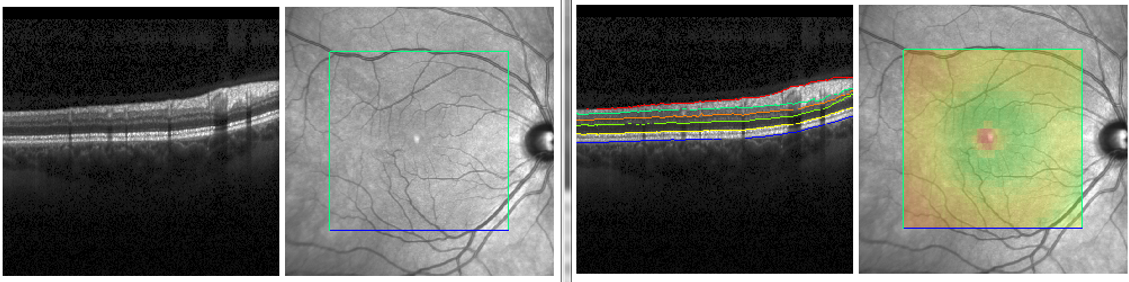
\includegraphics[width=0.8\textwidth]{fig/oct}
\end{center}
\caption{Optical Coherence Tomography (OCT) of retina layers segmentation: image data (left), image segmentation \& retina thickness map (right). \href{https://blog.surf.nl/eyr4-blog-7-lightpath-optical-coherence-tomography-oct-imaging/}{EYR4 project: Light-path for OCT imaging.}}
\label{fig:oct}
\end{figure}

Because of the complexity of the problem, the large number of imaging modalities, equipment and even image formats, usually specific algorithms are developed to segment different body organs and tissues. Since specific solutions are required, which are hard to generalize for other structures, modalities, even less across scientific domains, the image segmentation is left out of the scope of this report.


An example of the {\em identification} problem, is the individual photo-identification of wildlife. This is illustrated on Figure \ref{fig:photoid}. Many species are individually recognizable by characteristic patterns or shape, i.e. by their phenotype.


\begin{figure}[H]
\begin{center}
\includegraphics[width=0.8\textwidth]{fig/photoid}
\end{center}
\caption{Example species with sufficient spot pattering what could be useful for automated photo-identification: (a) whale shark (with reference area),
(b) spotted  tree frog, (c) northern quill, (d) Amazon spotted frog, (e) striped blue crow and (f) mangrove snake.}
\label{fig:photoid}
\end{figure}

An example of the {\em classification} problem is shown on Figure \ref{fig:woodphotoid}. The question is to identify the tree species from microscopic images of wood samples. The {\em Acer} has a different appearance than {\em Toona}, but also within the family there are many species of {\em Toona} which differ- for example {\em Toona ciliata} differs subtly from {\em Toona sinesis} (Figure \ref{fig:treeid}), hence the classification problem could be hierarchical and increasingly difficult.

\begin{figure}[H]
\begin{center}
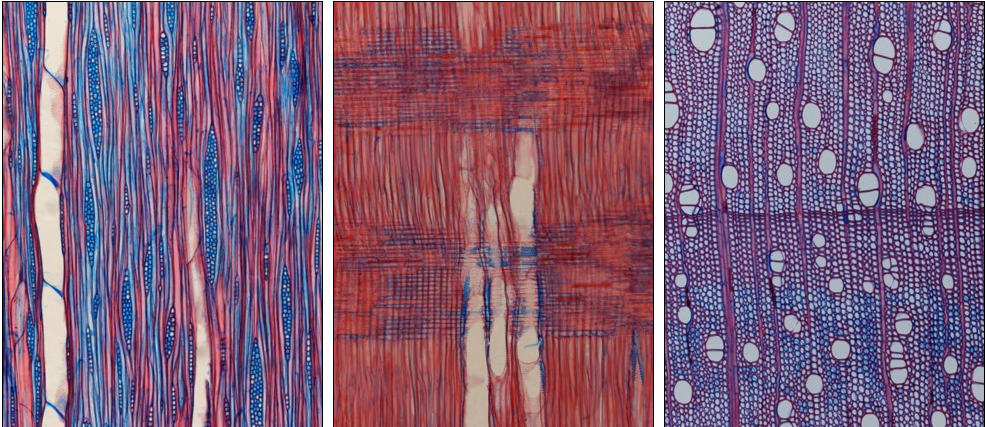
\includegraphics[width=0.8\textwidth]{fig/woodphotoid}
\end{center}
\caption{Left to right: tangential, radial and cross (transversal) sections of stained wood Acer.}
\label{fig:woodphotoid}
\end{figure}

\begin{figure}[H]
\begin{center}
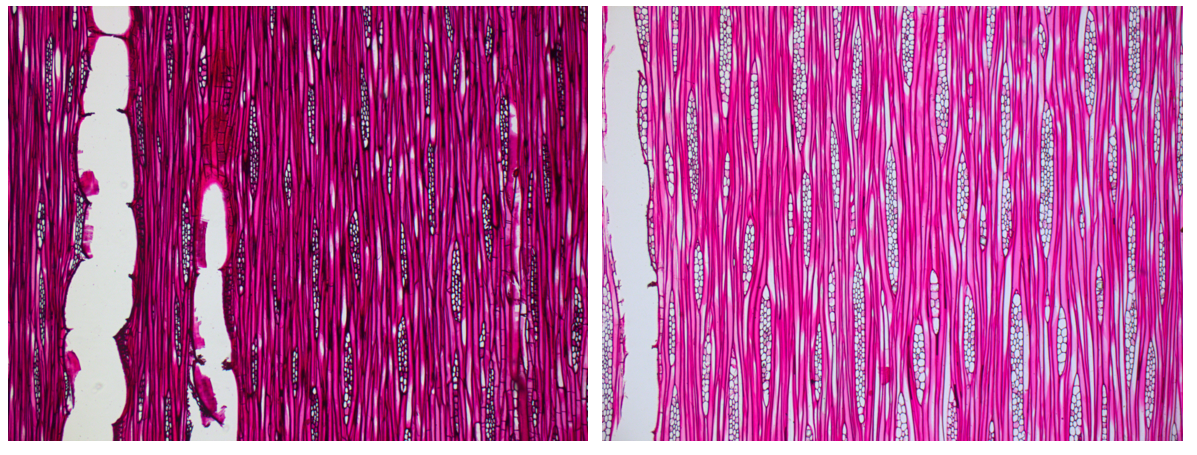
\includegraphics[width=0.8\textwidth]{fig/treeid}
\end{center}
\caption{Tangential section of stained wood. Left: Toona ciliata, Right: Toona sinesis.}
\label{fig:treeid}
\end{figure}

To address such scientific questions, three  CV\&IP research questions can be defined:
\begin{enumerate}
\item {\bf Visual salience:} How can the CV system determine automatically the most visual salient region(s) in an image?\label{item:sal}
\item {\bf Object/scene identification:} How can the CV system automatically determine whether two images, potentially taken with different cameras under different viewing conditions and transformations, represent the same object/scene?\label{item:ident}
\item {\bf Object/scene detection/classification:} How can the computer recognize automatically to what visual category the object/scene captured in an image belongs to? \label{item:und}
\end{enumerate}

There are also numerous non-scientific applications related to the above research questions.  For example {\em visual saliency} (\ref{item:sal}) in important in tasks such as:
\begin{itemize}
\item Automatic target detection (see Fig. \ref{fig:sal})
\item Robot navigation using salient objects
\item Image and video compression
\item Automatic cropping/centering images for display on small portable screens, etc.
\end{itemize}

\begin{figure}[H]
\begin{center}
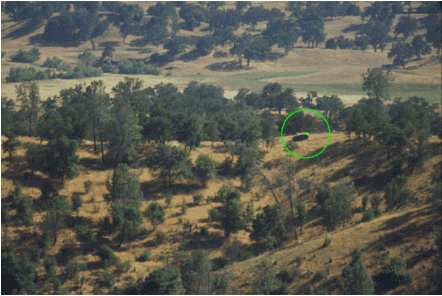
\includegraphics[width=0.8\textwidth]{fig/saliency}
\end{center}
\caption{Example of a saliency model detecting the vehicle as being the most salient object in a complex scene.}
\label{fig:sal}
\end{figure}


Few of the numerous applications related to {\em object/scene identification} (\ref{item:ident}) are:
\begin{itemize}
\item Stereo and wide-baseline matching
\item Image panorama stitching/creation
\item Automatic reconstruction of 3D scenes, etc.
\end{itemize}

Automatically understating the {\em semantics of an object/scene} (\ref{item:und}) in the form of image classification, have many applications like:
\begin{itemize}
\item Image search engines
\item Organizing photo collections
\item Autonomous driving
\item Human machine interaction
\item Digital forensic investigation, etc.
\end{itemize}

This is a complex and high-level computer vision task, with the goal of making machines see like humans and be able to infer both general principles as well as current situations from images. Example of a trained system for scene categorization is shown on Fig.\ref{fig:mitdemo}.
\begin{figure}[H]
\begin{center}
\includegraphics[width=0.8\textwidth]{fig/mitdemo}
\end{center}
\caption{ \href{http://places.csail.mit.edu/demo.html}{MIT Scene Recognition Demo.}}
\label{fig:mitdemo}
\end{figure}

In fact, the majority of CV\&IP researchers traditionally work on non-scientific applications, focusing on the third and most challenging problem. Addressing the problems faced by other domain scientist, while still conducting generic and widely applicable computer vision research, seems to fit best the strategy of NLeSc and eStep. 

The overview is by no means complete, it rather tries to summarize the research in the field along the above three questions in the last years. The report is structured along the main outputs of the CV\&IP research, namely, scientific publications in Section \ref{sec:pubs}, software in Section \ref{sec:soft} and datasets in Section \ref{sec:db}. Some potential scientific applications are shown in Section \ref{sec:app}. The conclusions and recommendations are given is section \ref{sec:conc}.
\section{Publications}
\label{sec:pubs}


\subsection{Saliency}

In \cite{LiuCVPR2007} the salient object detection is formulated as image segmentation problem. The object is separated from the background on the basis of several features including multi-scale contrast, center-surround histogram and colour spatial distribution for the object description on several levels- locally, regionally and globally. The multi-scale contrast is the local feature, the center-surround histogram is the regional feature and the colour spatial histogram- the global. These features are illustrated on Figure \ref{fig:sal_feat_liu07}.
\begin{figure}[H]
\begin{center}
\includegraphics[width=0.95\textwidth]{fig/SalientFeatures_Liu2007}
\end{center}
\caption{Examples of salient features. From leftto right: input image, multi-scale contrast, center-surround histogram, colour spatial distribution and binary salient mask by CRF.}
\label{fig:sal_feat_liu07}
\end{figure}
A conditional Random Field is trained on these features. 
For the purposes of this research the autors have compiled a large-scale database, MSRA (\cite{msra_db}), presented in section \ref{subsec:msra}. The database is publically available, while the software is not. The proposed methods compared to two other algorithms ``FG" (fuzzy growing) and ``SM" (salient model as computed by the SalientToolbox, described in section \ref{subsec:saltool}). The authors' tends to produce smaller and more focused bounding boxes.

{\em good for automatic cropping?}
In \cite{LCAV-CONF-2009-012} the authors perform a frequency-domain analysis on five stateof-
the-art saliency methods, and compared the spatial frequency
content retained from the original image, which is
then used in the computation of the saliency maps. This
analysis illustrated that the deficiencies of these techniques
arise from the use of an inappropriate range of spatial frequencies.
Based on this analysis, they presented a frequency-tuned
approach of computing saliency in images using low
level features of color and luminance. The resulting saliency maps are better suited to salient object segmentation, with higher precision and
better recall than the analyzed state-of-the-art techniques.

In \cite{YanCVPR2013} the authors address a fundamental problem in saliency detection, namely, the small-scale background structures, which affect the detection. This problem occurs often in natural images. They propose a hierarchical framwork that infers importance values fromimage layers with different scales. The approach is summarized in Figure \ref{fig:hier_yan13}.

\begin{figure}[H]
\begin{center}
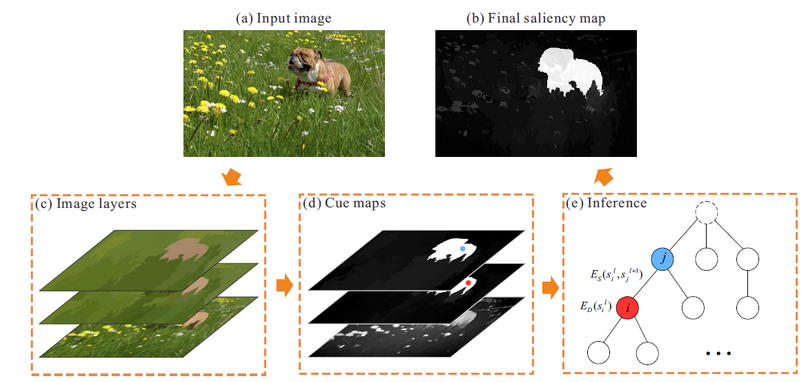
\includegraphics[width=0.95\textwidth]{fig/Hierarchy_Yan13}
\end{center}
\caption{An overview of the hierarchical framework. Three image layers are extracted from the input, and then  saliency cues from each of these layers are computed. They are finally fed into a hierarchical model to get the final results.}
\label{fig:hier_yan13}
\end{figure}

For the purpose of their research the authors made a new database available to the community, the Complex Scene Saliency dataset (CSSD) and the Extended CSSD (ECSSD), described in Section \ref{subsec:cssd}. The executable of their software is also available from the project link (\cite{ecssd_db}), but not the source code. The authors report better performence of their method on MSRA-1000 and (E)CSSD datasets comapred to $11$ other state-of-the-art methods.

\subsection{Salient regions}

In \cite{Forssen07} colour extension ot the popular {\em  Maximally Stable Extremal Regions (MSER)} detector is proposed. The author calles his detector {\em Maximally stable colour region (MSCR)}. In comparision on the well-known Visual Geometry Group in Oxford test image sets (\cite{vgg_soft_data}) with known homographies to the original MSER detector, the simple colour MSER extension (MSER3) and a colour blob detector, the MSCR performes better in most cases. The executables of the software for MSCR and blob detectors are available at the author's homepage \cite{forssen07_soft}.

The MSER detectorhas been also extended in 3D to {\em Maximally Stable Volumes (MSVs)} in \cite{DonoserB06}. The MSVs have been used to sucessfully segment 3D medical images and paper fiber networks.

In \cite{Fan08} a structure-guided salient region detector (SGSR) is introduced. It is based on entropy-based saliency theory and shows competitive performance.

In \cite{Wang14} another enhancmenet of MSER is proposal, namely with Canny detector....

\subsection{Convolutional Neural Networks}
\section{Software}
\label{sec:soft}

The saliency detection, dataset annotation and recognition tools developed by the researchers are often made available to the community.

\subsection{Saliency}
\subsubsection{SaliencyToolbox}\label{subsec:saltool}
The SaliencyToolbox is a collection of Matlab functions and scripts for computing the saliency map for an image, for determining the extent of a proto-object, and for serially scanning the image with the focus of attention. 

\subsubsection{Frequency-tuned Saliency}
The code used in the CVPR 2009 paper ``Frequency-tuned Salient Region Detection'' (\cite{LCAV-CONF-2009-012}) is accessible through the online presentation of the work at \cite{achantaCVPR09}.

\subsection{Dataset annotation}
\subsubsection{LabelMe}\label{subsec:labelme}
\cite{Russell2008}
\section{Datasets}
\label{sec:db}

The annotated segmentation and saliency datasets, which are used by the researchers to test the algorithms are often made available to the object saliency detection and segmentation community.

\subsection{Saliency Datasets}
\subsubsection{MSRA}
The MSRA  Database form the Visual computing group of Microsoft  research \cite{msra_db} is a collection of two image sets. The first set consists of $20 000$ images labeled by three users, while the second set consists of $5000$ images labeled by nine users. The labeling are available as bounding boxes. Figure \ref{fig:msra} illustrates the dataset.
\begin{figure}[H]
\begin{center}
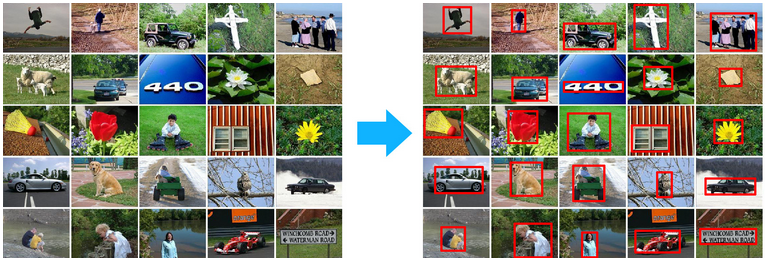
\includegraphics[width=0.95\textwidth]{fig/MSRA}
\end{center}
\caption{Examples of the MSRA dataset.}
\label{fig:msra}
\end{figure}
\subsubsection{MSRA10k}
This is an extension of the MSRA dataset, which  addresses the coarse-grained limitation of the MSRA labeling (bounding boxes). The MSRA10k (\cite{msra10k_db}) dataset consists of $10000$ randomly selected MSRA images for which a pixel-level saliency labeling is available. Figure \ref{fig:msra10k} illustrates the dataset. 
\begin{figure}[H]
\begin{center}
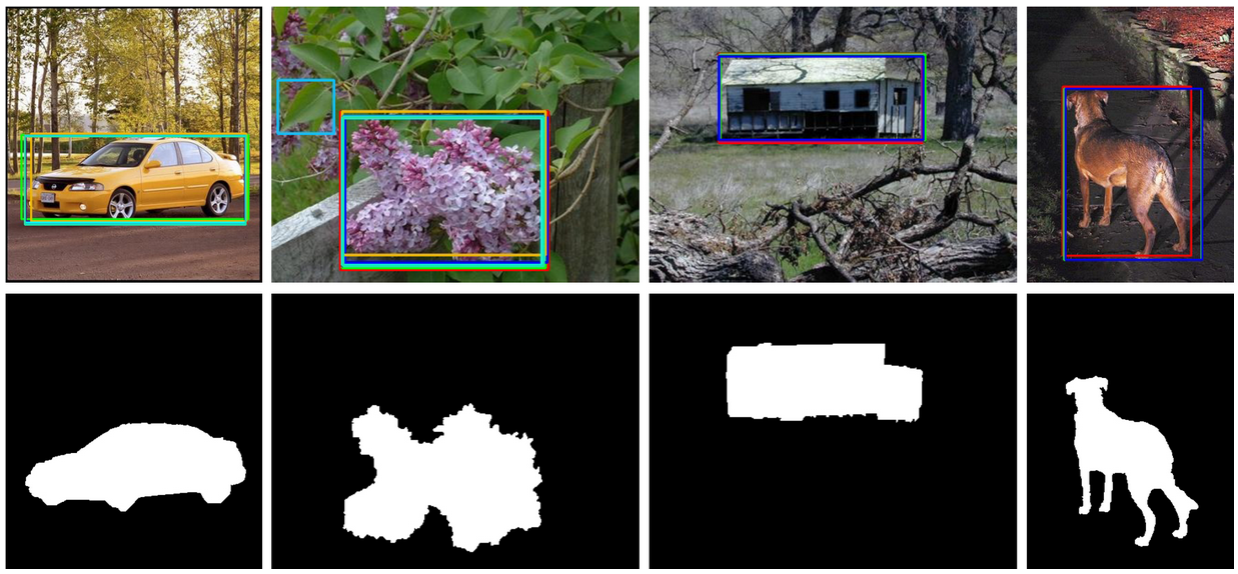
\includegraphics[width=0.95\textwidth]{fig/MSRA10k}
\end{center}
\caption{Examples of the MSRA 10k dataset. First row: original images with ground truth rectangles from MSRA dataset. Second row: Ground truth with pixel accuracy.}
\label{fig:msra10k}
\end{figure}
This dataset is used by in a very recent paper in IEEE Transactions on PAMI \cite{ChengPAMI2015} and \cite{chengPAMIUrl} (online resources with link to the software). 

\subsubsection{CSSD and ECSSD}
Although images from MSRA-1000 \cite{LCAV-CONF-2009-012} have a large variety in their content, background structures are primarily simple and smooth. To represent the situations that natural images generally fall into, the Complex Scene Saliency Dataset (CSSD) \cite{cssd_db} was proposed in \cite{YanCVPR2013} with $200$ images. They contain diverse patterns in both foreground and background. The labeling has done by five  helpers. These images were collected from the BSD300 (later extended to BSD500, \cite{bsd300/500_db}), VOC dataset \cite{voc_db} and internet.

Later, the CSSD was extended to a larger dataset (ECSSD) of $1000$ images, which includes many semantically meaningful and structurally complex images for evaluation. The images are acquired from the internet and five helpers were asked to produce the ground truth masks. Examples of the images in the dataset can be seen on Figure \ref{fig:ecssd}.

\begin{figure}[h]
\begin{center}
\includegraphics[width=0.95\textwidth]{fig/ECSSD}
\end{center}
\caption{Examples of the ECSSD dataset.}
\label{fig:ecssd}
\end{figure}

\subsection{DUT-OMRON}
The datasets mentioned so far, although widely used in the community are not {\em large-scale} per se. The Dalian University of Technology and the Omron Corporation introduced in the DUT-OMRON dataset \cite{dut-omron_db} consisting of $5168$, manually selected from more than $140 000$ images. They are re-sized to $400 \times x$ or $x \times 400$, where  $x < 400$. They contain one or more salient objects with relatively complex background. Five people have labeled the pixel-wise ground truth along with bounding box and eye-fixation. The dataset is illustrated on Figure \ref{fig:dut-omron}. The results of the experiments on the collected dataset were published in \cite{yang2013saliency}.

\begin{figure}[h]
\begin{center}
\includegraphics[width=0.75\textwidth]{fig/DUT-OMRON}
\end{center}
\caption{Samples of the DUT-OMRON dataset.From top to bottom: original image, bounding box ground truth, pixel-wise ground truth,average of the five binary masks and eye-fixation ground truth. }
\label{fig:dut-omron}
\end{figure}

\subsection{PASCAL-S}
Another dataset, which aims at bridging the gap between fixations and salient objects is the PASCAL-S dataset \cite{pascal-s_db} provided by Georgia Tech, Caltech and UCLA. The dataset contains $850$ images from the PASCAL 2010 with $12$ subjects and $1296$ object instances. The images and the code are available for download. The dataset is is illustrated on Figure \ref{fig:pascal-s}.

\begin{figure}[H]
\begin{center}
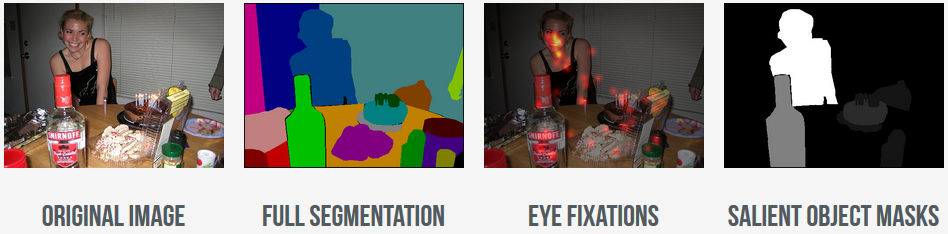
\includegraphics[width=0.95\textwidth]{fig/PASCAL-S}
\end{center}
\caption{Examples of the PASCAL-S dataset.}
\label{fig:pascal-s}
\end{figure}


The saliency segmentation method and the findings have been published at \cite{TPAMI.2012.147}.  

\section{Applications}
\label{sec:app}

In any scientific discipline, where for studying the object of research, the scientist need to process (large scale) image/video datasets, CV technology can be applied.  For many decades, CV techniques have been applied widely and become standard tool in many scientific applications. Examples are remote sensing (imaging Earth of pa planet), electrical resistivity imaging (geophysical method to image the underground), sonar and radar imaging, and one of the most important applications- (bio)medical imaging. Here, only a few examples of recently emerging application domains are given, even more new challenges will appear when scientists from different domains become aware of the capabilities and potential of the CV technology.

\subsection{Animal biometrics}
\label{sec:anim_biom}
In \cite{Kuehl2013}, Kuehl and Burghardt give overview of the methodologies and trends in the emerging field of {\em animal biometrics}. It is an exciting field operating at the intersection between pattern recognition, ecology and information sciences. The subject of the field is to produce computerized systems for phenotypic measurement and interpretation. The main questions for which such systems helps to find the answers to are: how to profile species, individuals and animal behavior by representing phenotypic appearance. Figure \ref{fig:photoIDpen} illustrates the main components of a biometric system. 

\begin{figure}[H]
\begin{center}
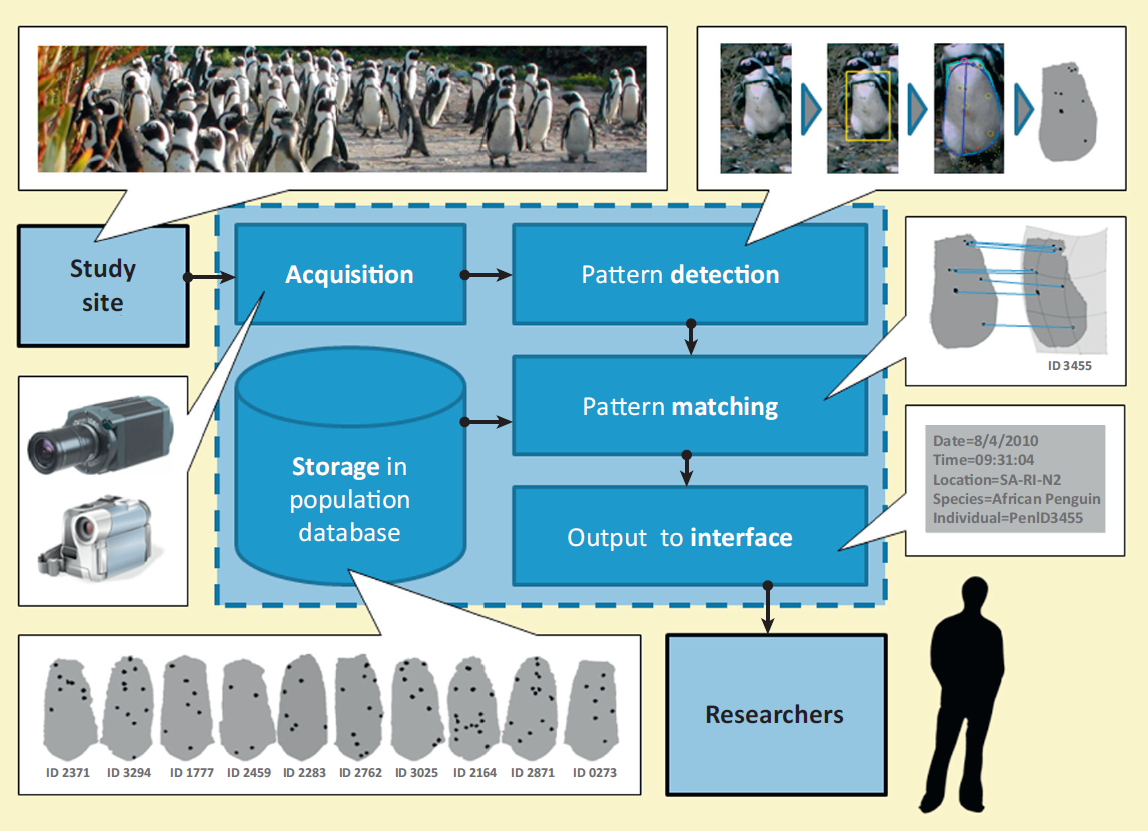
\includegraphics[width=0.68\textwidth]{fig/PhotoIDPenguins}
\end{center}
\caption{Main components of an animal biometric system. This flowchart summarizes how information from a study site is measured and interpreted for the researcher by
an animal biometric system.}
\label{fig:photoIDpen}
\end{figure}
The system parts can either be connected directly on-site or remotely via networks. Each of the components is illustrated, using individual African penguin recognition by spot pattern as an example.  Acquisition: automatic or semi-automatic collection of images or video from fixed field cameras, observers or
the general public. Detection: the use of computer algorithms to search the images to find those that contain the biometric entity of interest and then to extract relevant
information about that entity (e.g., the chest spots of a penguin). Storage: the extracted data on the entity is reduced to a compact mathematical form that can be stored in a
suitable database. Matching: the mathematical data on the entity are then compared with other data already stored in the database to find matches that enable the
individual or the behavior to be identified, using methods akin to the matching of fingerprints to identify humans. Interfacing: presenting the output of the biometric system
to a user or software system for further analysis.

Animal biometrics is important field not only for ecological researchers, but for the general public. For example, in \cite{Kumar2014}, a biometric system for face recognition of pet animals (mainly dogs) have been developed.

\subsection{Plant identification}
Similar field is automatic plant identification. This is an example of the Classification task (What is my object?). Often the identification of trees and flowers is performed from images of the leaves of the plant. Nowadays, many \href{http://www.gardenista.com/posts/diy-identify-leaves-and-flowers-theres-an-app-for-that}{\underline{mobile app}s} exist for the general public.

One such CV system is \href{http://neerajkumar.org/projects/leafsnap/}{\underline{Leafsnap}}, \cite{leafsnap}. Its goal is to assist botanists by automating the tedious and error-prone process of identifying existing plant species. 

The recognition process, developed by the research groups from Columbia University and University of Maryland, consists of, \cite{leafsnap_eccv2012}:
\begin{enumerate}
\item{ {\bf Segmenting} the image to obtain a binary image separating the leaf from the background. This is implemented using an Expectation-Maximization framework, estimating foreground and background color distributions in the HSV color-space.}
\item{{\bf Extracting features} from the binarized image for compactly and discriminatively representing the shape of the leaf. The features used are histograms of curvature over scale as the feature representation, robustly and efficiently implemented using integral measures of curvature.}
\item{{\bf Comparing the features} to those from a labeled database of leaf images and returning the species with the closest matches. Due to the discriminative power of the features and the size of our labeled dataset, we use a simple nearest neighbor approach with the $L_1$-norm.}
\end{enumerate}
The system has the same components as that of an animal biometric system (Figure \ref{fig:photoIDpen}), which indicates, that plan biometrics is a very similar application domain to animal biometrics.

Figure \ref{fig:Leafsnap} gives an impression of the functionality of Leafsnap.

The example of tree species identification (see the \underline{\nameref{sec:intro}} section) is another problem from the same domain. Also, in a the current NLeSC project \href{https://www.esciencecenter.nl/project/prediction-of-candidate-genes-for-traits-using-interoperable-genome-annotat}{\underline{candYgene}} image-based classification of different tomato species collected from different places in the world could be applied. 
\begin{figure}[H]
\begin{center}
\includegraphics[width=0.95\textwidth]{fig/LeafSnap}
\end{center}
\caption{Tour of the iPhone version of Leafsnap.}
\label{fig:Leafsnap}
\end{figure}



\subsection{Computer forensics}
{\em  Forensic Science} is the application of knowledge from several branches of science to answer questions relevant to a legal system. Due to the evolution of criminal activities, more
specialized disciplines have been involved, such as Computer Science, Engineering and Economics.
The research field that unites the fields of Forensic Science and Computer Science is called {\em Computer (Digital) Forensics} and encompasses the study of research methods, driven by
hypothesis, of a specific problem, through the use of computers and computational methods.

Many questions in digital forensics can be answered (or assisted) by CV technologies, such as face detection and identification, same object/scene identification, image/video categorization, camera identification etc. for which the presented earlier CV methods are very highly applicable.

There are also specific problems for example, photogrammetry, 3D  reconstruction  of  impressions, reconstruction of fragmented documents and images etc. Research is done in novel CV methods which help solve these problems, \cite{Andalo13SIBGRAPI}.

\subsection{Social signal processing}
In the last years, a multi-disciplinary area, called {\em Social  Signal  Processing} emerged where computer vision and social sciences converge.  One of the research topics is the development of video surveillance  algorithms to help studying social interactions. Technologically the problems are those of gesture (frequency) analysis, gait, pose and emotion recognition, geometric configuration of people, etc. (Figure \ref{fig:SSP}). A survey of this domain with presentation of the main applications and research results can be found in \cite{Vinciarelli:2009}. 

\begin{figure}[H]
\begin{center}
\includegraphics[width=0.75\textwidth]{fig/SSP}
\end{center}
\caption{Behavioral cues and social signals. Multiple behavioral cues (vocal behavior, posture, mutual gaze, interpersonal distance, etc.) combine to produce a social signal
(in this case aggressivity or disagreement).}
\label{fig:SSP}
\end{figure}


\href{http://www.measuringbehavior.org/}{\underline{\em Measuring behavior }} is the premier interdisciplinary event for scientists and practitioners concerned with the study of human or animal behavior. The biannual conference is held traditionally in the Netherlands. At the same time, the CV community becomes more aware of these applciaiton areas, for example one \href{http://www.seas.upenn.edu/~hypar/GroupBehavior/cvpr15_tutorial_group_behavior.html}{\underline{tutorial}} at the Computer Vision ad Pattern Recognition (CVPR) conference 2015 was on ``Group Behavior Analysis and Its Applications''.
\section{Conclusions}
\label{sec:conc}

To goal of  this document was to present focused study of the state-of-the-art in (large-scale) computer vision research. The reader should have a general overview and find useful pointers to where one might direct research and development efforts. It is also important to know the current trends in the field to be able to sustain some level of expertise in it.

Based on researching the articles, software, the ever growing number of research image datasets and the (scientific) application domains few main concussions crystallize:

\begin{itemize}
\item{CV field is very large and fast changing. More and more scientific disciplines pose new challenges to CV. To sustain some level of expertise in it, NLeSc should conduct (scientific-driven) CV research, for example within eStep.}
\item{The research efforts should focus around the relevant research questions, presented in the document: localization, identification and classification. Given the current expertise, it is very reasonable to continue improving the MSSR salient region detector (see section \underline{\fullref{subsec:salreg}}). Also, some expertise should be build in Convolutional neural networks (section \underline{\fullref{subsec:cnn}}) by organizing seminars and obtaining practical knowledge for example within project Sherlock.}
\item{The CV researchers in academia are focused mostly on large commercial applicators like organizing large photo collections, autonomous driving, etc. There is still not enough effort directed towards the other domain sciences (except from the medical imaging) where NLeSC can contribute (section \underline{\fullref{sec:app}}). Also, sustaining expertise in large scale frameworks for CV systems (section \underline{\fullref{subsec:largescale}}) fits very well the mission and strategy of the center.}
\item{Although not covered by this overview, at NLeSC we see the appearance of new modality, the Point clouds, by which the real world is captured in a way which removes some of the limitations of CV mentioned in the \fullref{sec:intro}. For example in Patty project, methods from CV have been applied to generate PC from images. There is a research in trying to identify objects directly from the PC and it is interesting to find out can the CV algorithms be applied directly on PC or new or adapted algorithms are needed.}

\end{itemize}



\bibliographystyle{plain}
\bibliography{bibliography}

\end{document}

